\documentclass[11pt]{article} 
\usepackage{calc, tikz}
\usepackage[margin={1in,1in}]{geometry} 
\usepackage[hwkhandout]{hwk}
\usepackage[pdftitle={Calc 1
  Notes},colorlinks=true,urlcolor=blue]{hyperref}

\renewcommand{\theclass}{\textsc{math}1300: calculus I}
\renewcommand{\theauthor}{Tyson Gern}
\renewcommand{\theassignment}{Parametric Equations}
\renewcommand{\dateinfo}{section 4.8}

\newcommand{\ds}{\displaystyle}

\begin{document}
\drawtitle

\begin{enumerate}
\item The motion of a particle on the $xy$-plane is given by
  \begin{align*}
    x(t) &= t^3 - \frac{3}{2}t^2 - 6t\\
    y(t) &= t^3 - \frac{9}{2}t^2 + 6t.\\
  \end{align*}

  \begin{enumerate}
  \item Does the particle ever come to a complete stop?  If so, when
    and where?
    \vfill
  \item Is the particle ever moving straight up or down?  If so, when
    and where?
    \vfill

    \newpage
    
  \item Is the particle ever moving straight horizontally right or
    left?  If so, when and where?
    \vfill
  \end{enumerate}

\item Find the equation of the tangent line to the parametric equation
  \begin{align*}
    x(t) &= t^2\\
    y(t) &= t^3
  \end{align*}
  at $t = 2$. Write your answer as a parametric equation.
  \vfill
  \newpage
  
\item Two particles move in the $xy$-plane.  At time $t$, the position
  of a particle $A$ is given by
  \begin{align*}
    x(t) &= 4t-4 & y(t) &= 2t-k,\\
    \intertext{and the position of particle $B$ is given by}
    x(t) &= 3t & y(t) &= t^2-2t-1.
  \end{align*}

  \begin{enumerate}
  \item If $k=5$ do the particles ever collide?  Explain.
    \vfill
  \item Find $k$ so that the two particles do collide.
    \vfill

    \newpage
    
  \item Using the $k$-value from part (b), which particle is moving
    faster when they collide.
    \vfill
  \end{enumerate}

\item The figure below shows the graph of the parametric curve
  \begin{align*}
    x(t) &= f(t)\\
    y(t) &= f'(t),
  \end{align*}
  for a function $f(t)$.
    \begin{center}
      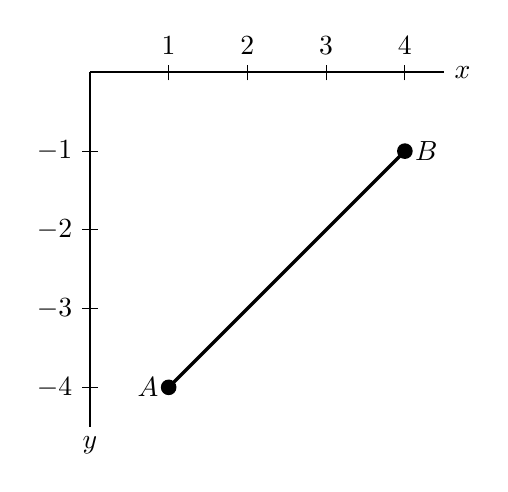
\begin{tikzpicture}
        \def\xmin{-0}\def\xmax{5} \def\ymin{-5}\def\ymax{0} 
        \foreach \i in {\xmin,...,4} {\ifnum\i=0{}
          \else{\draw
            (\i,-.1) -- (\i,.1) node[above] {$\i$};}\fi}
        \foreach \i in {-4,...,\ymax} {\ifnum\i=0{}
          \else{\draw
            (.1, \i) -- (-.1, \i) node[left] {$\i$};}\fi}
        
        \draw[thick] (\xmin,0) -- (4.5,0) node[right] {$x$}; \draw[thick] (0,0) --
        (0,-4.5) node[below] {$y$};
        
        \draw[very thick] (1,-4) -- (4,-1);
        \draw [thick, fill=black] (1,-4) circle [radius=0.085] node[left]{$A$};
        \draw [thick, fill=black] (4,-1) circle [radius=0.085] node[right]{$B$};
    \end{tikzpicture}
  \end{center}

  \begin{enumerate}
  \item Is $f(t)$ an increasing or decreasing function?
    \vfill

    \newpage
    
  \item As $t$ increases, is the curve traced from $A$ to $B$ or from
    $B$ to $A$?
    \vfill
  \item Is $f(t)$ concave up or concave down?
    \vfill
  \end{enumerate}

  \newpage

\item A particle moves in the $xy$-plane so that its position at time
  $t$ is given by
  \begin{align*}
    x(t) &= \sin(t)\\
    y(t) &= \cos(2t)
  \end{align*}
  for $0\leq t \leq 2\pi$.
  \begin{enumerate}
  \item At what time does the particle first touch the $x$-axis? What
    is the speed of the particle at that time?
    \vfill
  \item Is the particle ever at rest?
    \vfill
  \item Discuss the concavity of the graph.
    \vfill
  \end{enumerate}


\end{enumerate}

\end{document}
